\documentclass[10pt]{report}
% define the title
\usepackage[brazil]{babel}
\usepackage[utf8]{inputenc}		%Usar acentos diretos do teclado
\usepackage[T1]{fontenc}		%Padrão para imagens
\usepackage{graphicx}
\usepackage{subfigure}
\usepackage{rotating}
\usepackage{longtable}
\usepackage{amsmath}
\usepackage{amsfonts}
\usepackage{amssymb}
\usepackage{geometry}
\usepackage{caption}
\geometry{left=3cm, right=2cm, top=2cm, bottom=2cm}
% Title Page
\title{Relatório Unidade 3 - Circuitos para Comunicação - Obtenção de Constelação e Cálculo da BER em Sistema RF de Modulação QPSK}
\author{Pedro Yochinori Gushiken}



\begin{document}
\maketitle
\chapter{Constelação - Experimento 1}
\section{Diagrama}
Geramos os dados a serem transmitidos a partir de um bloco no Advanced Design System(ADS), que é um software usado para Design de Sistemas de RF, Micro-ondas e Sistemas Digitais de Alta Velocidade. Os dados gerados passam por um Splitter que os divide entre as vias I e Q. Ao entrar nas vias são multiplicados por cossenos defasados entre si de $90^o$. Ao final as vias I e Q são somadas novamente. Este é o esquema básico da modulação PSK em quadratura. Neste primeiro experimento não introduzimos ruídos nem atenuação no canal, de forma que o resultado esperado é uma constelação QPSK "limpa" com 4 pontos distintos e perpendiculares entre si.
\begin{figure}
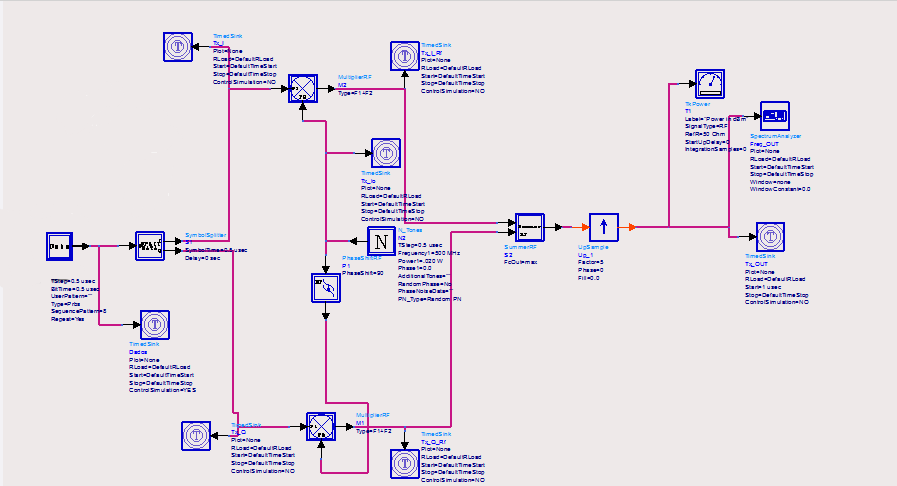
\includegraphics[width=.7\linewidth]{./primeiro_exp/1.png}
\caption{Diagrama de Blocos Referente ao Primeiro Experimento}
\end{figure}


\section{Resultados}

Obtivemos os resultados esperados na simulação, a saída do somador RF é uma boa representação dos dados gerados na entrada do modulador, as vias I e Q são de fato perpendiculares entre si. A constelação QPSK é basicamente a esperada, como explicado na legenda da figura.


\begin{figure}
\centering
\begin{minipage}{.48\textwidth}
  \centering
  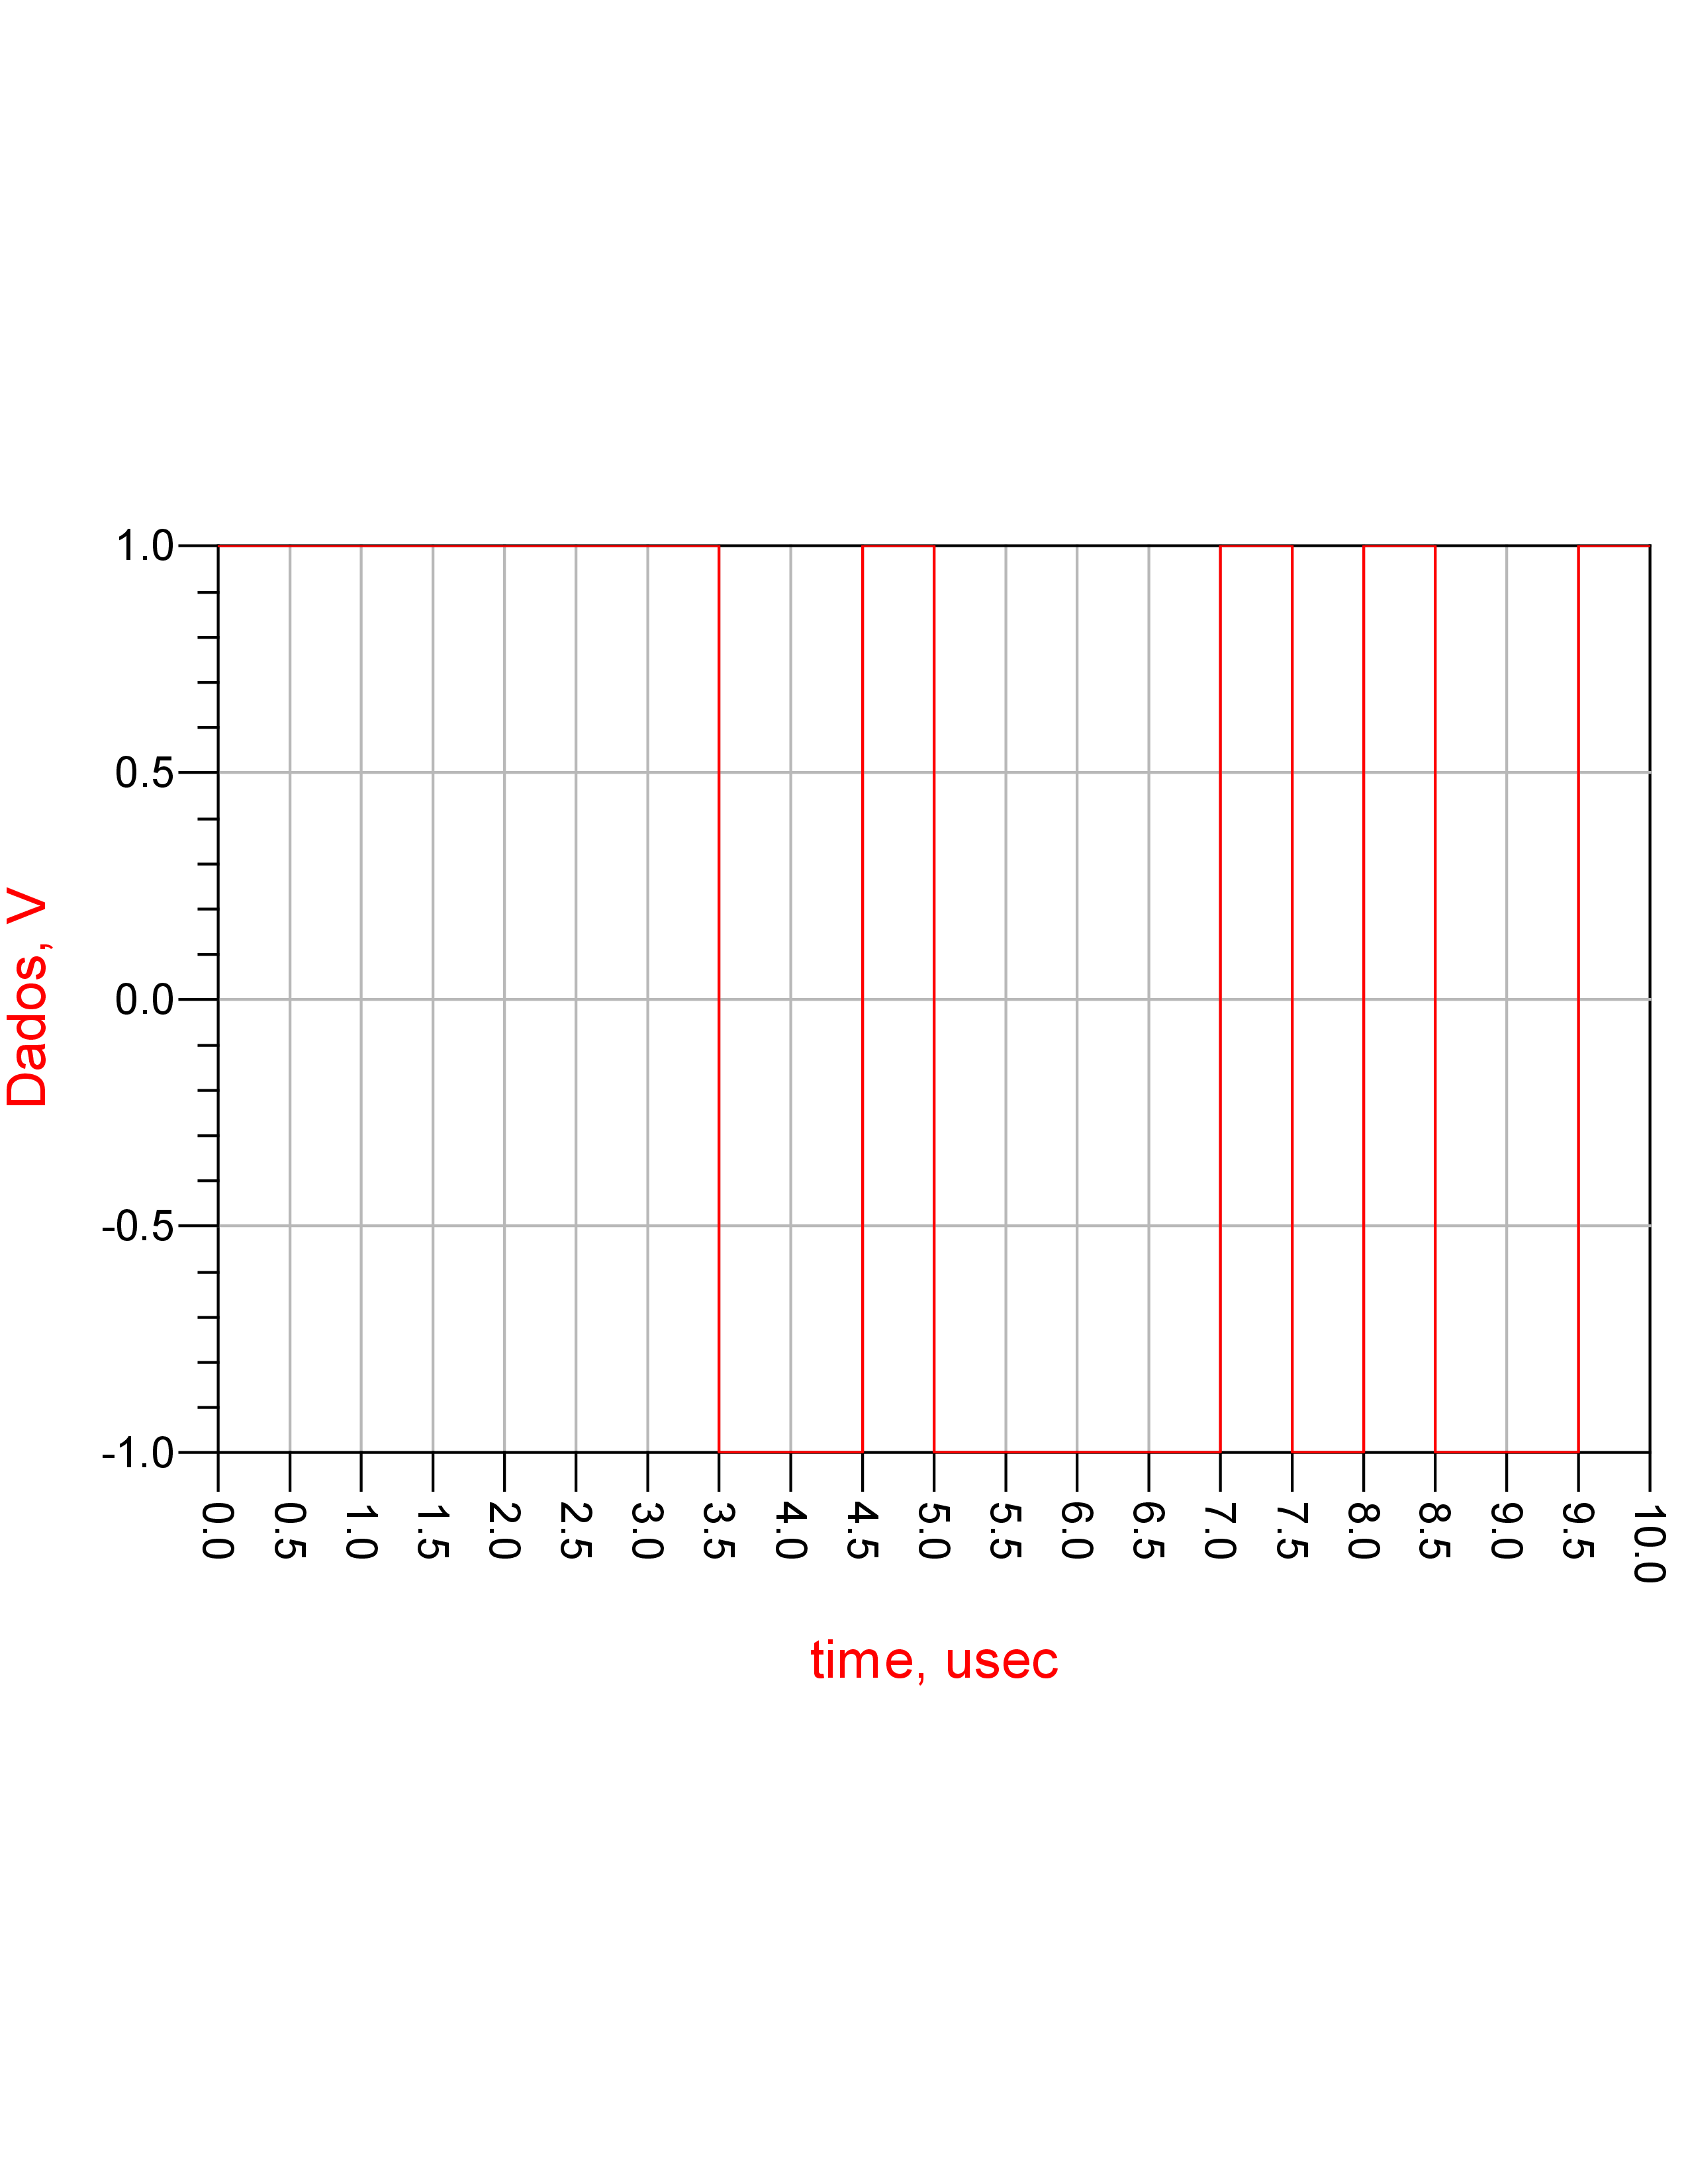
\includegraphics[width=\linewidth]{./primeiro_exp/img3.png}
  \captionof{figure}{Dados Gerados}
  \label{fig:test32}
\end{minipage}%
  \hfill
\begin{minipage}{.48\textwidth}
  \centering
  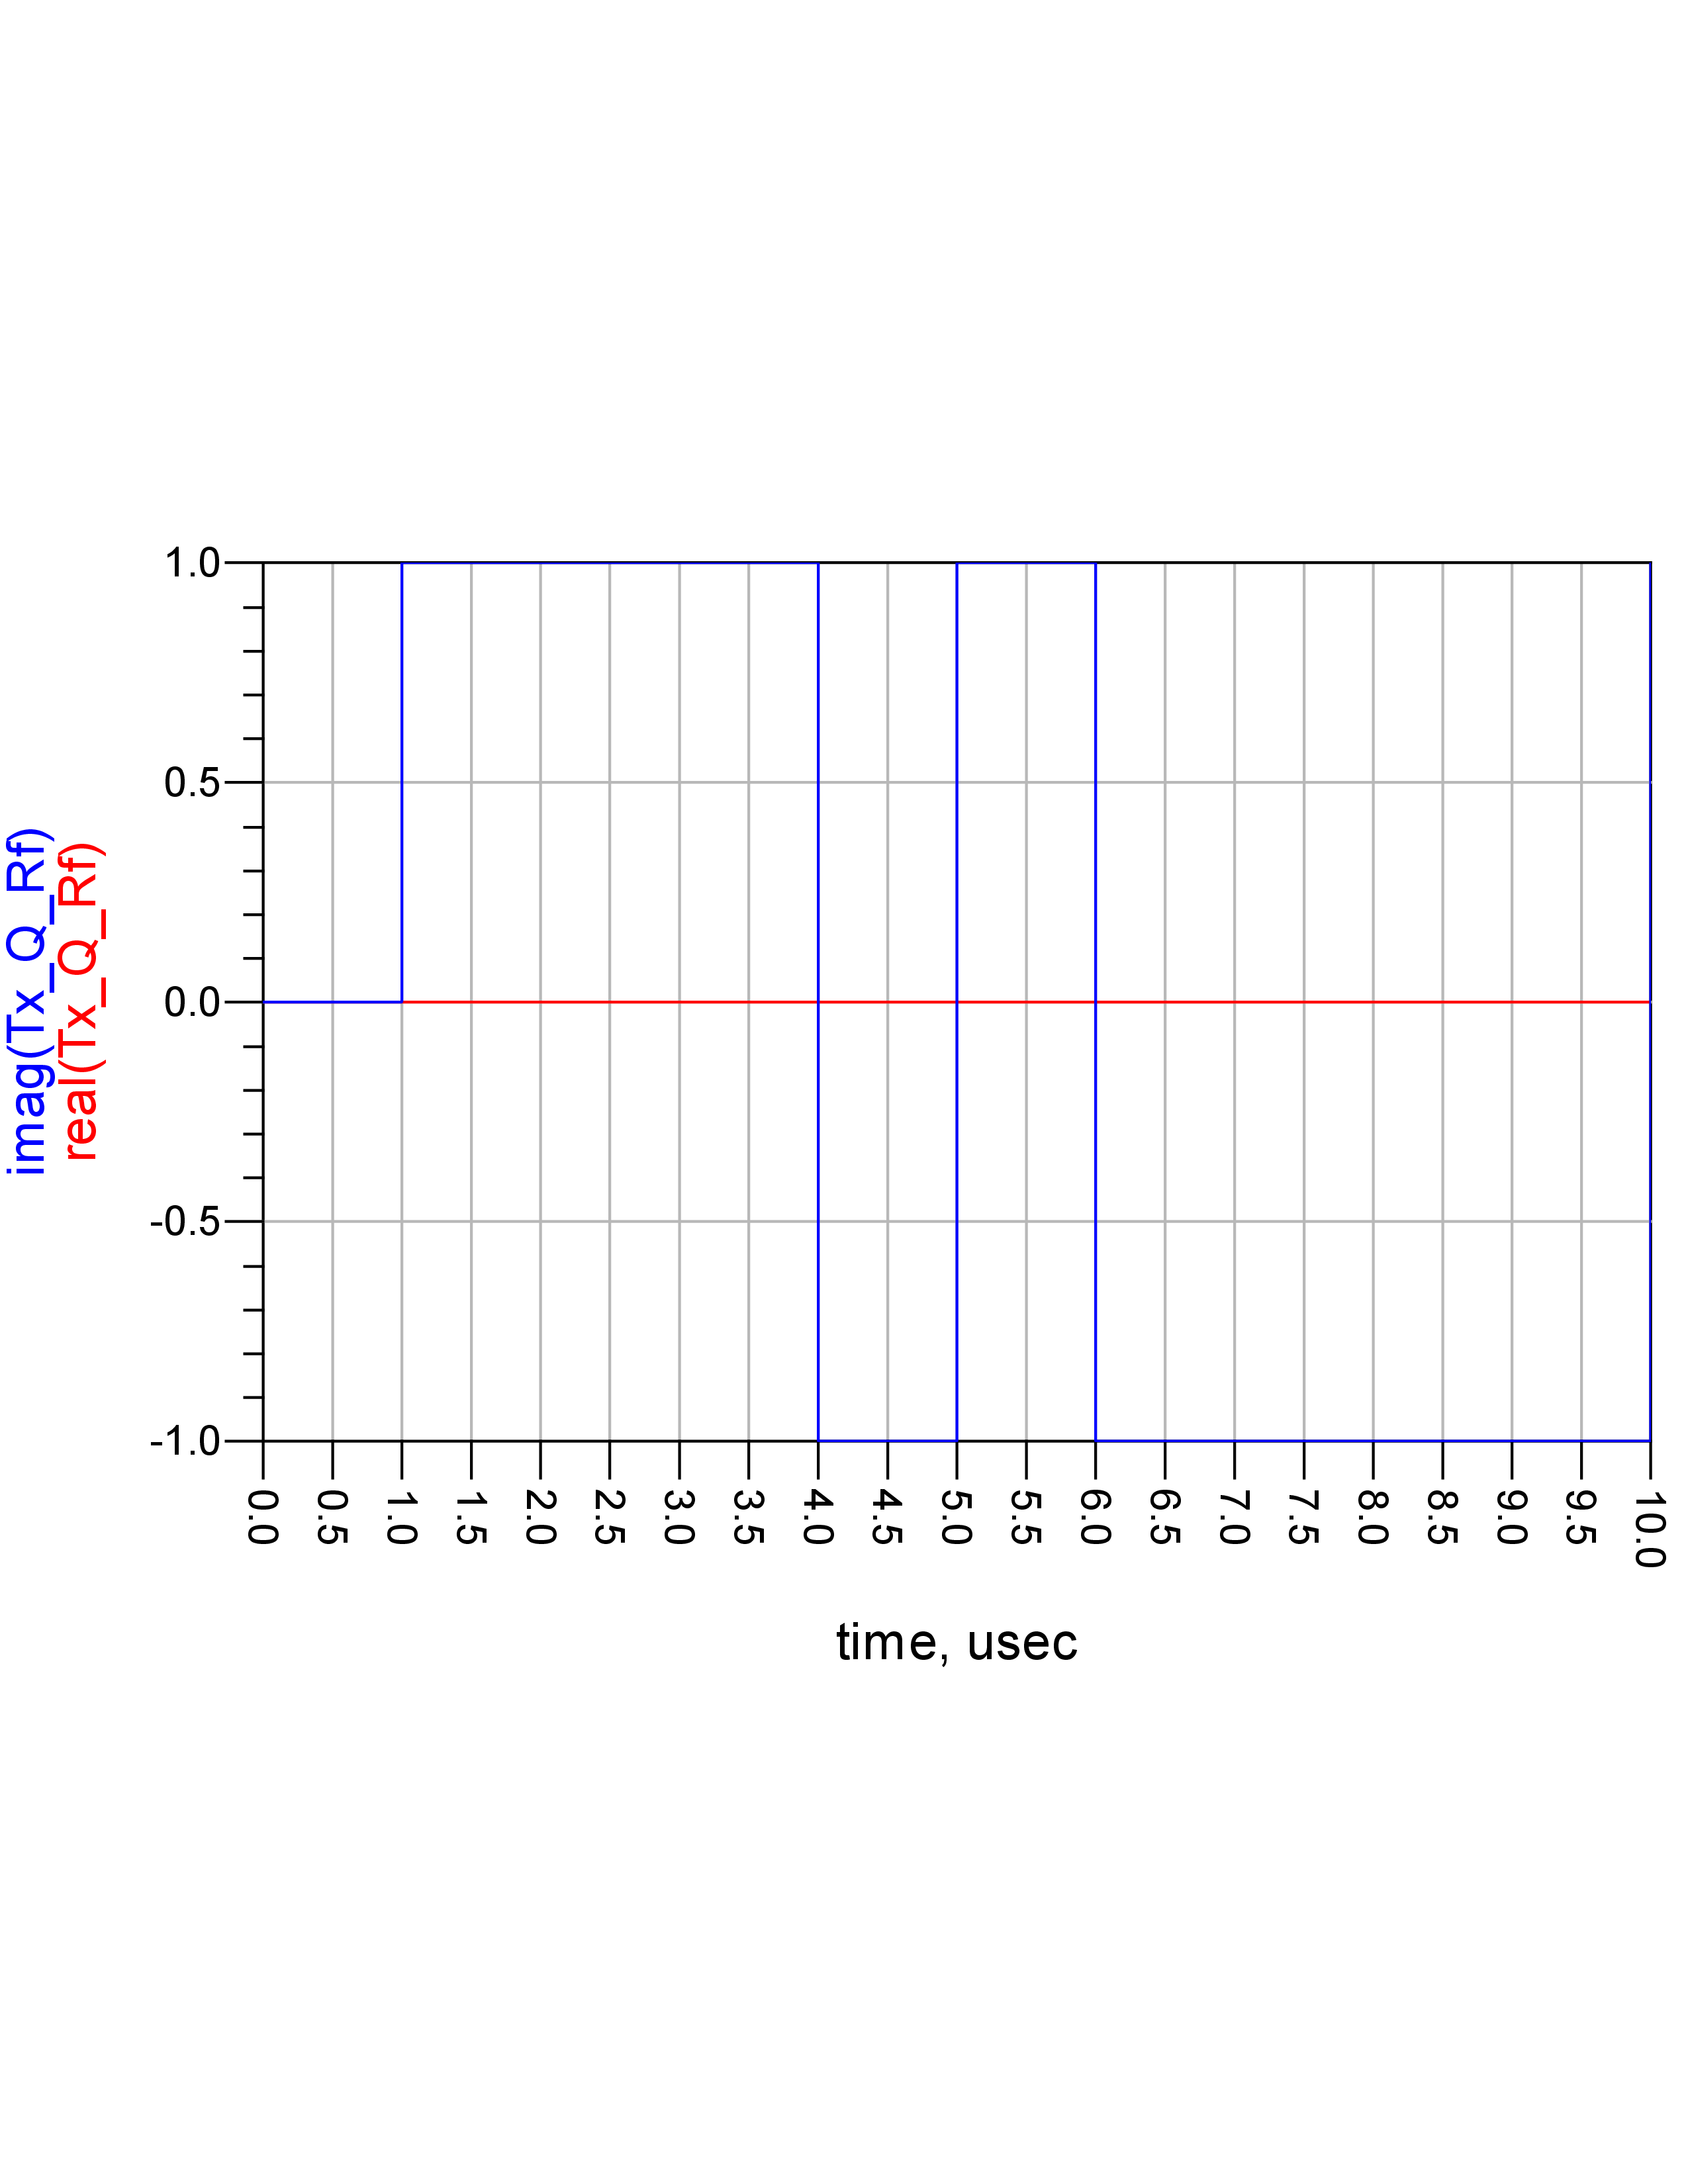
\includegraphics[width=\linewidth]{./primeiro_exp/img5.png}
  \captionof{figure}{Via Q, Parte Real e Imaginária}
  \label{fig:test43}
\end{minipage}
\end{figure}

\begin{figure}
\centering
\begin{minipage}{.48\textwidth}
  \centering
  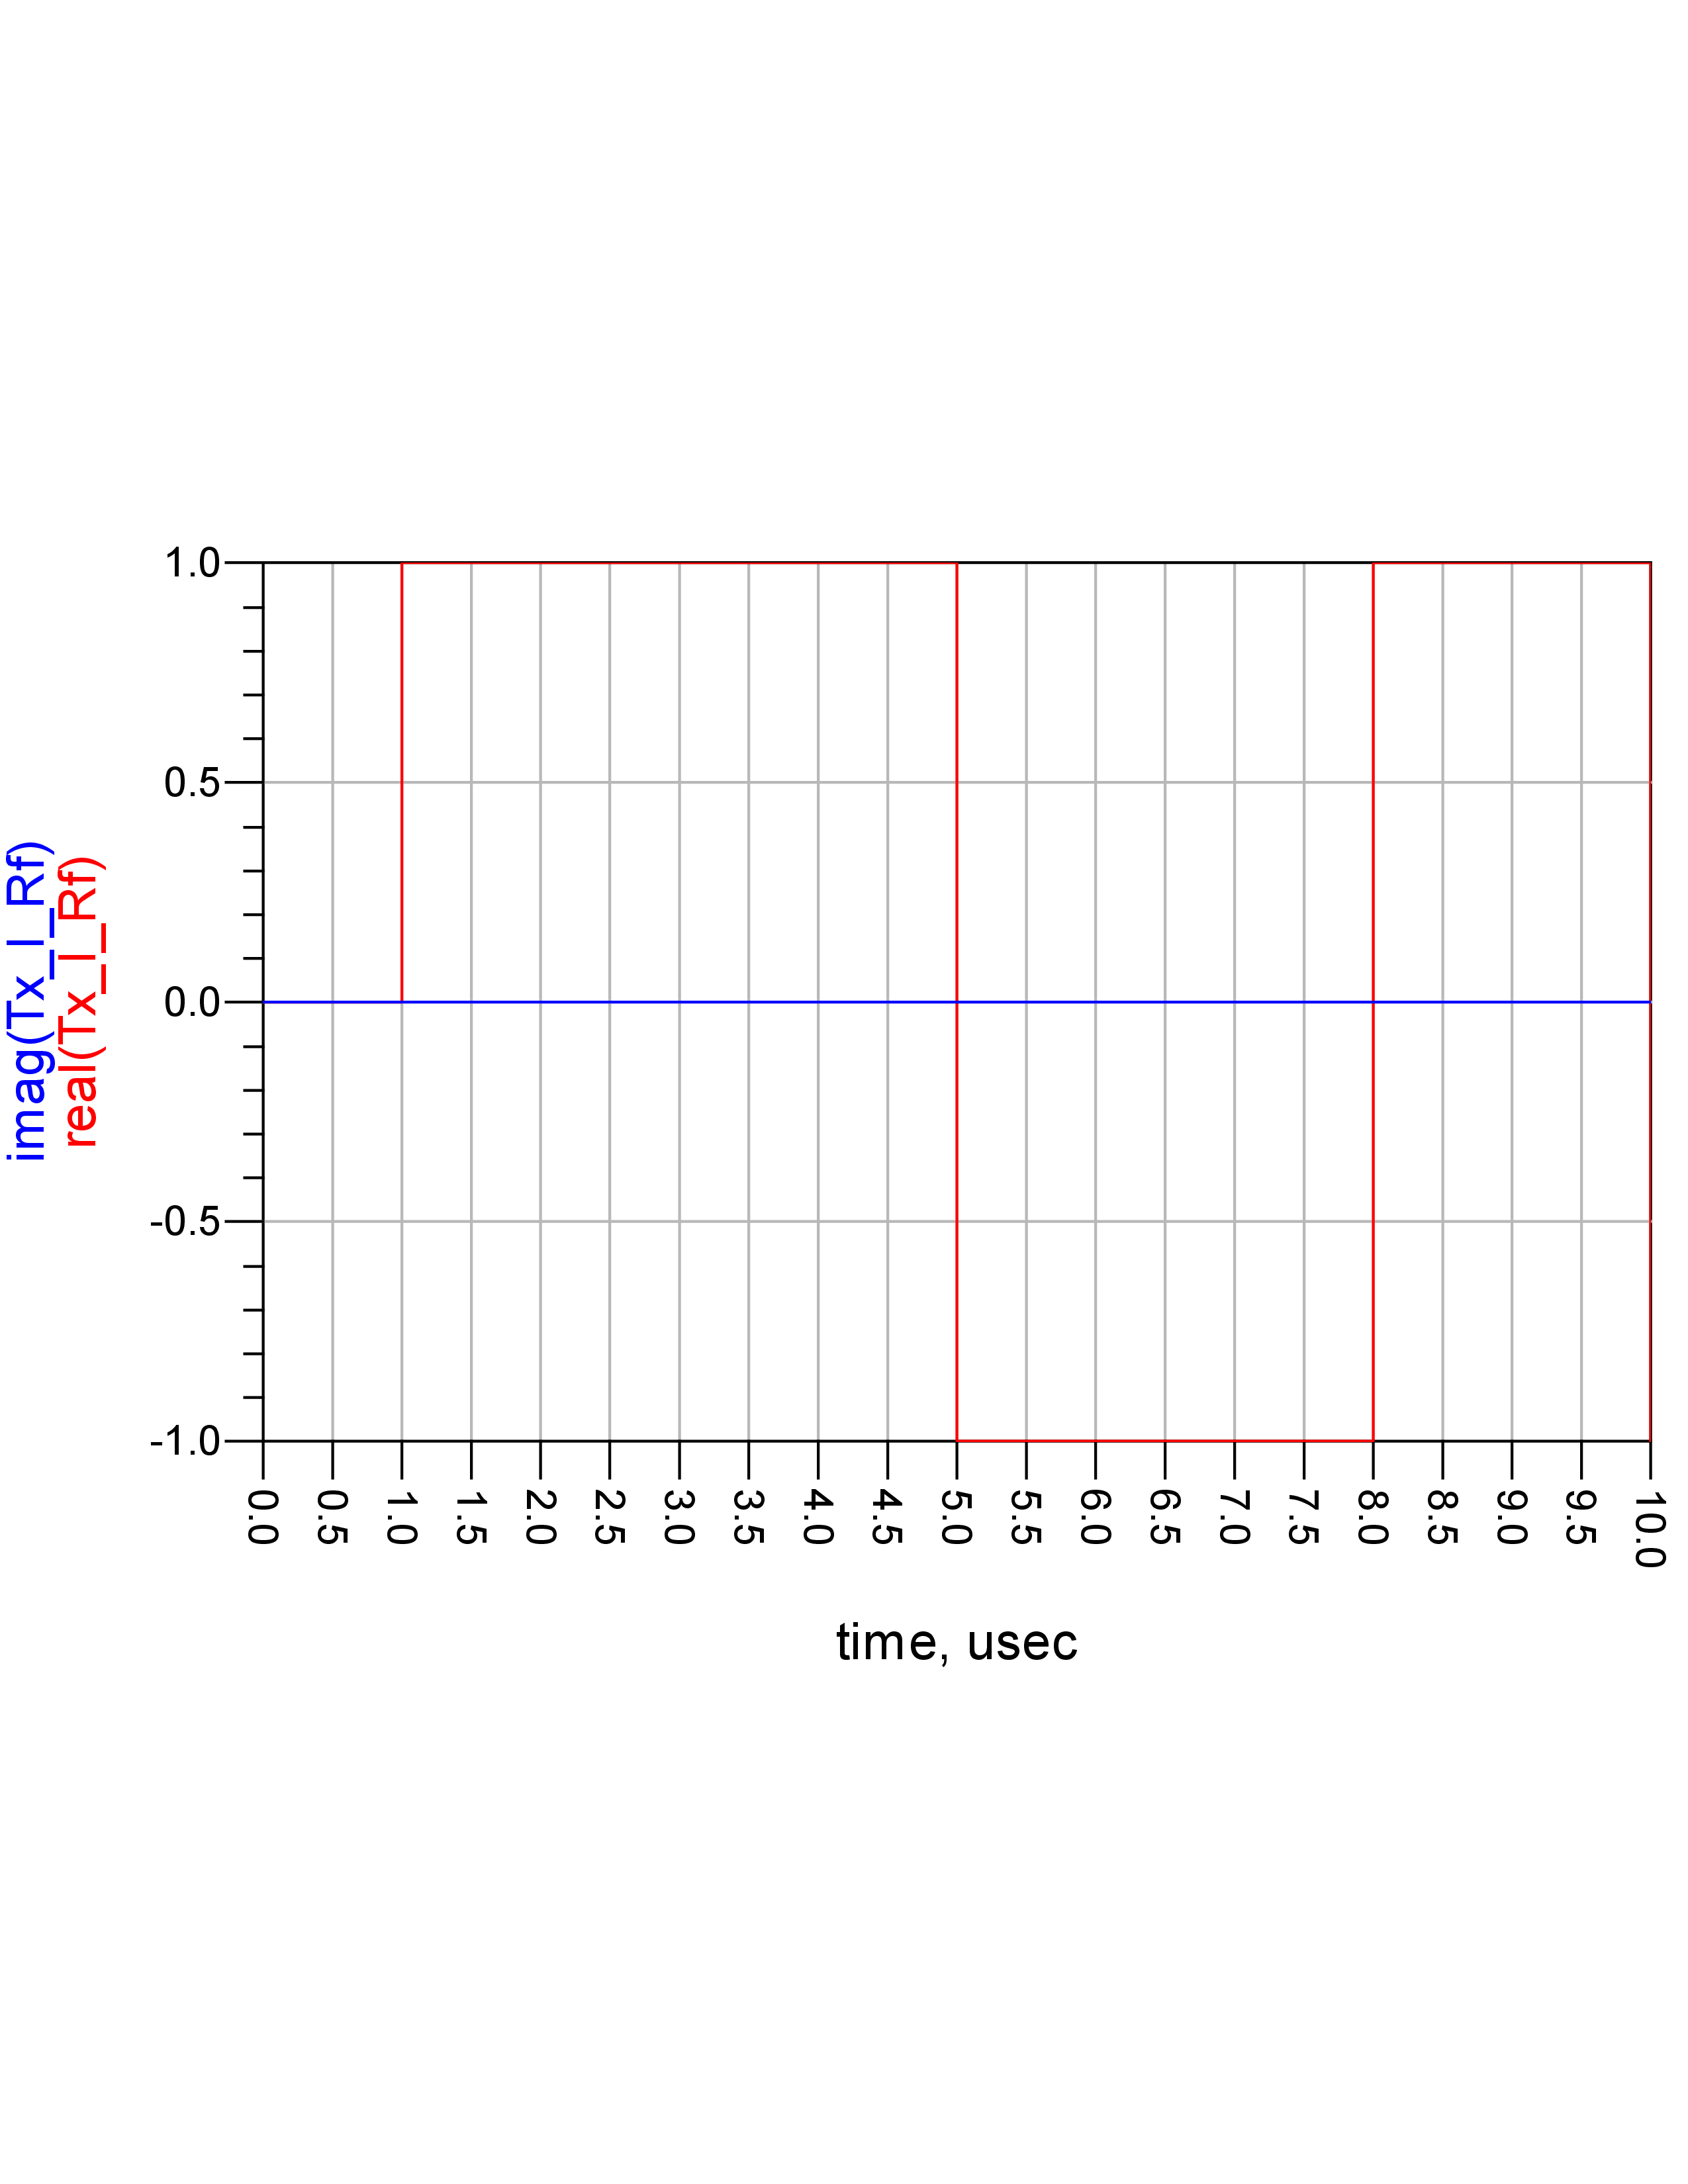
\includegraphics[width=\linewidth]{./primeiro_exp/img4.png}
  \captionof{figure}{Via I, Parte Real e Imaginária}
  \label{fig:test31}
\end{minipage}%
  \hfill
\begin{minipage}{.48\textwidth}
  \centering
  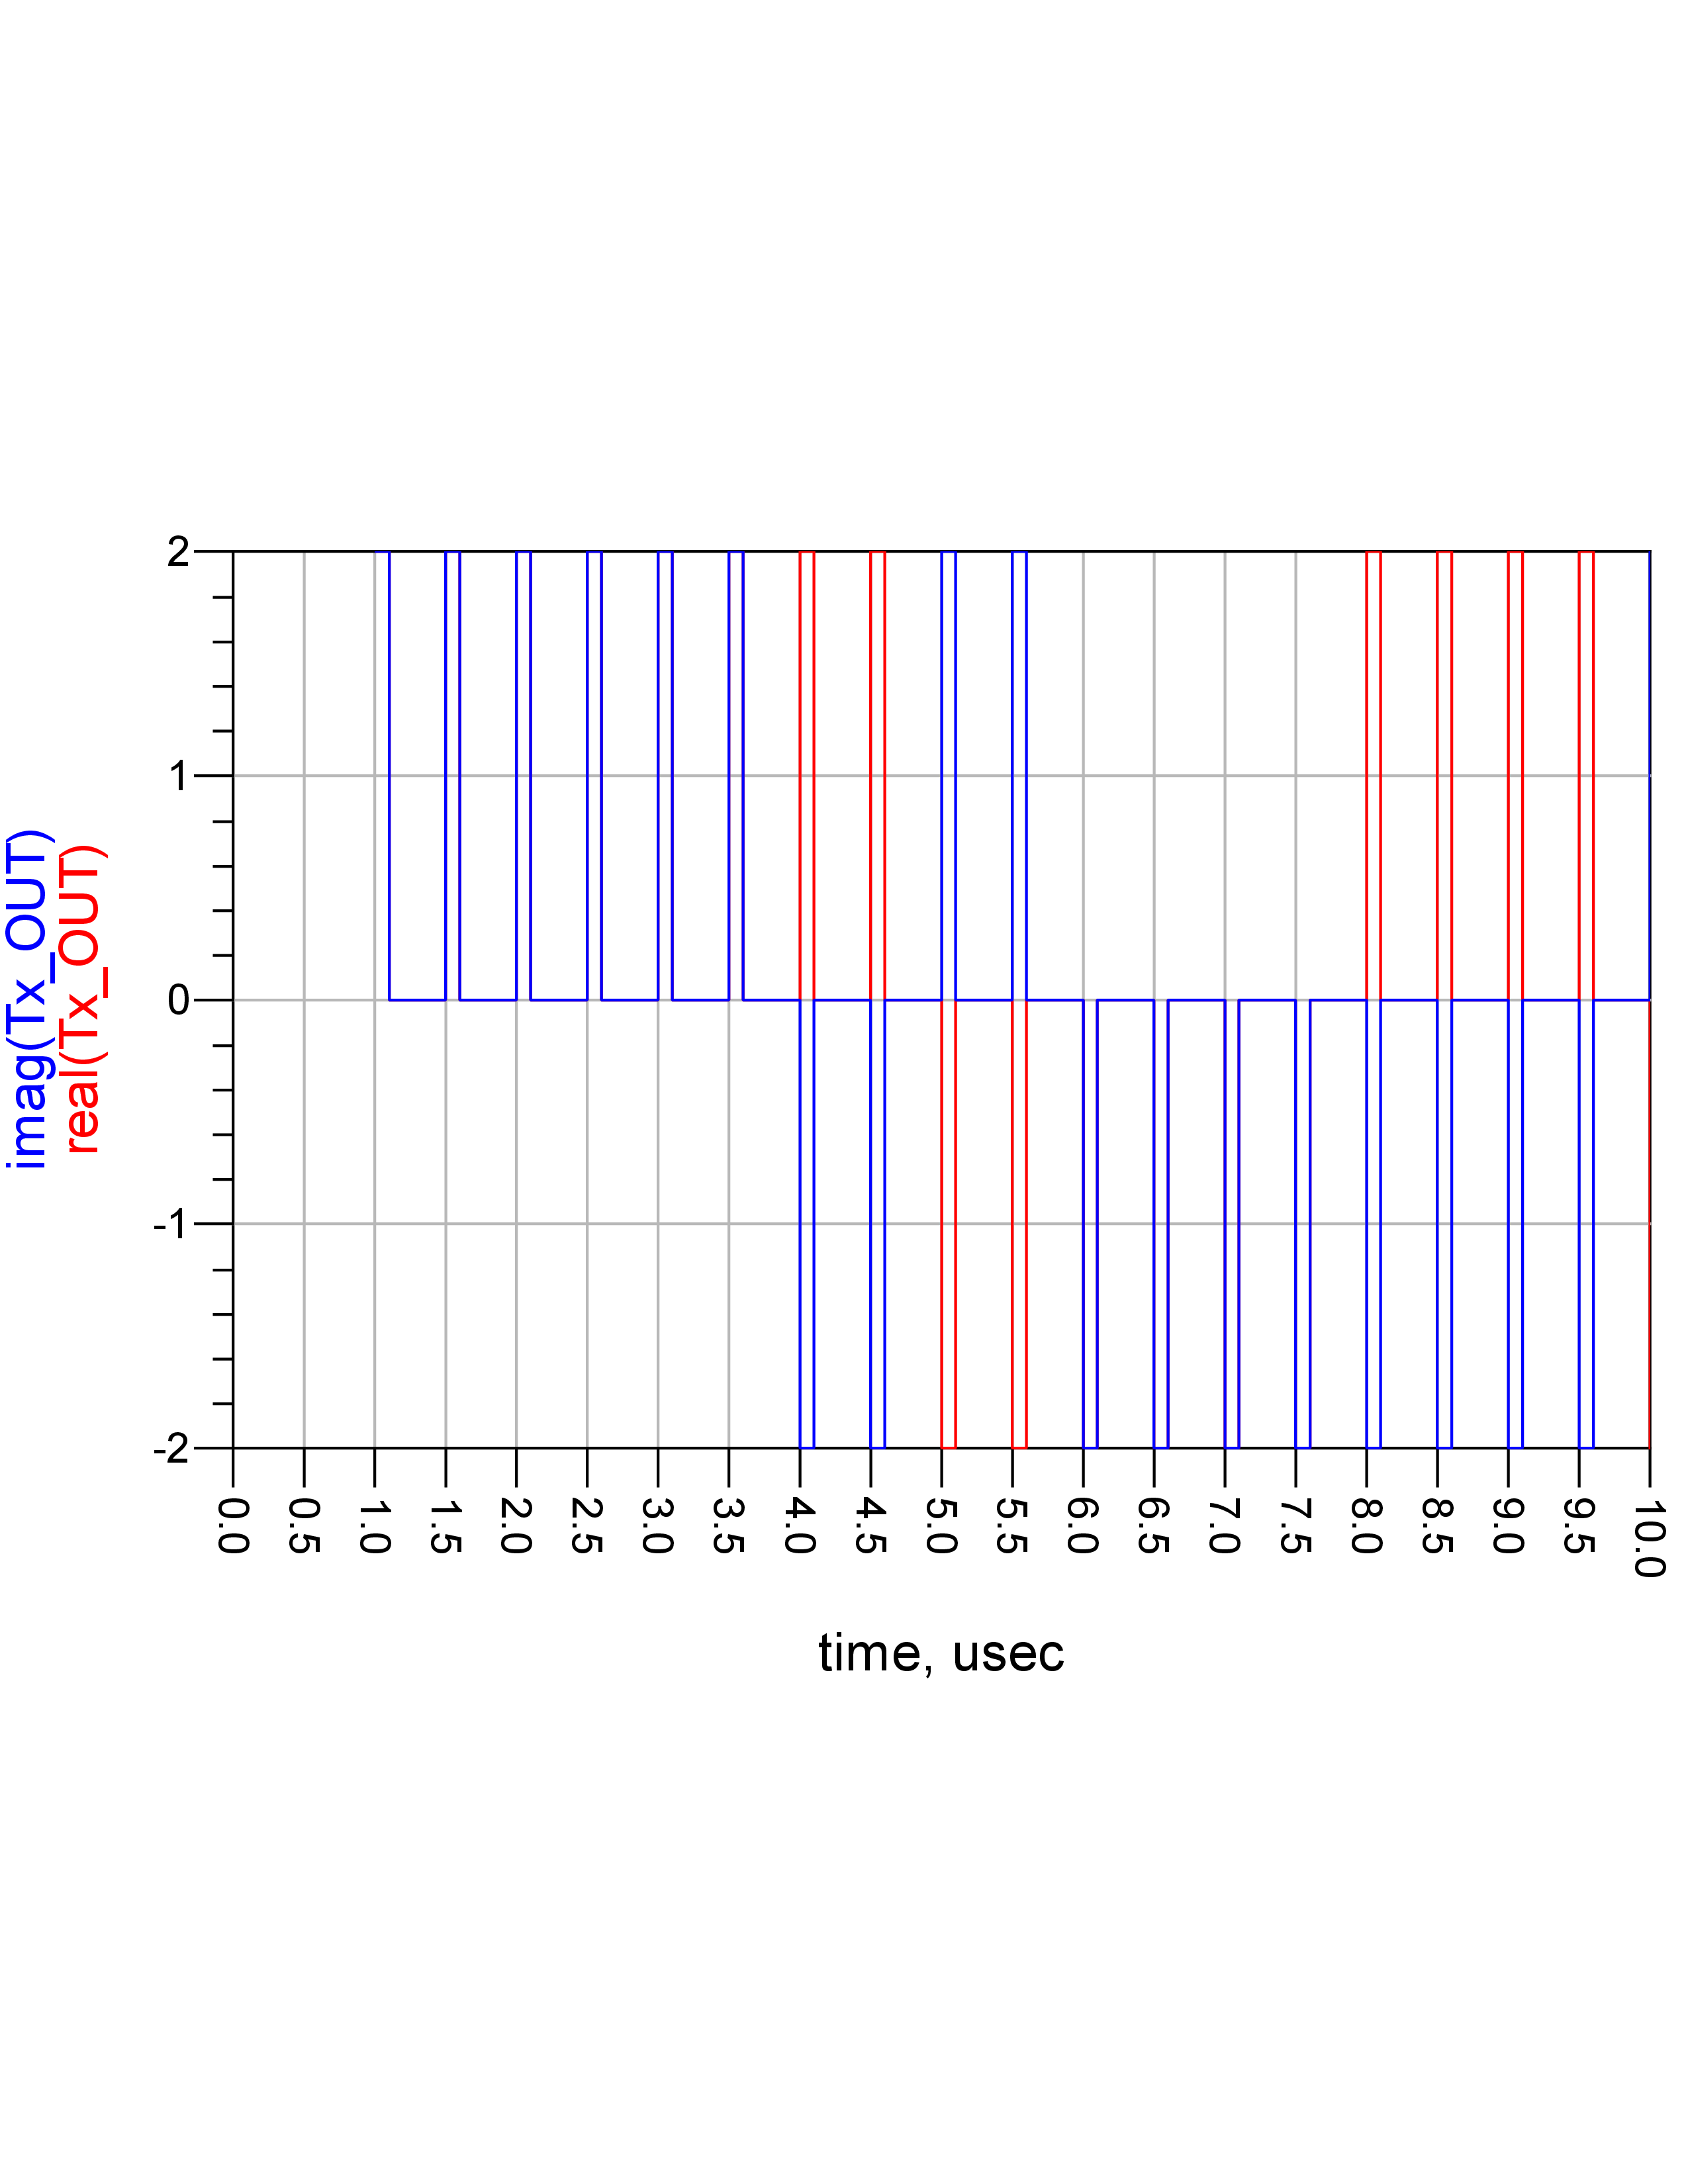
\includegraphics[width=\linewidth]{./primeiro_exp/img6.png}
  \captionof{figure}{Saída do Somador RF, Parte Real e Imaginária}
  \label{fig:test41}
\end{minipage}
\end{figure}
\begin{figure}
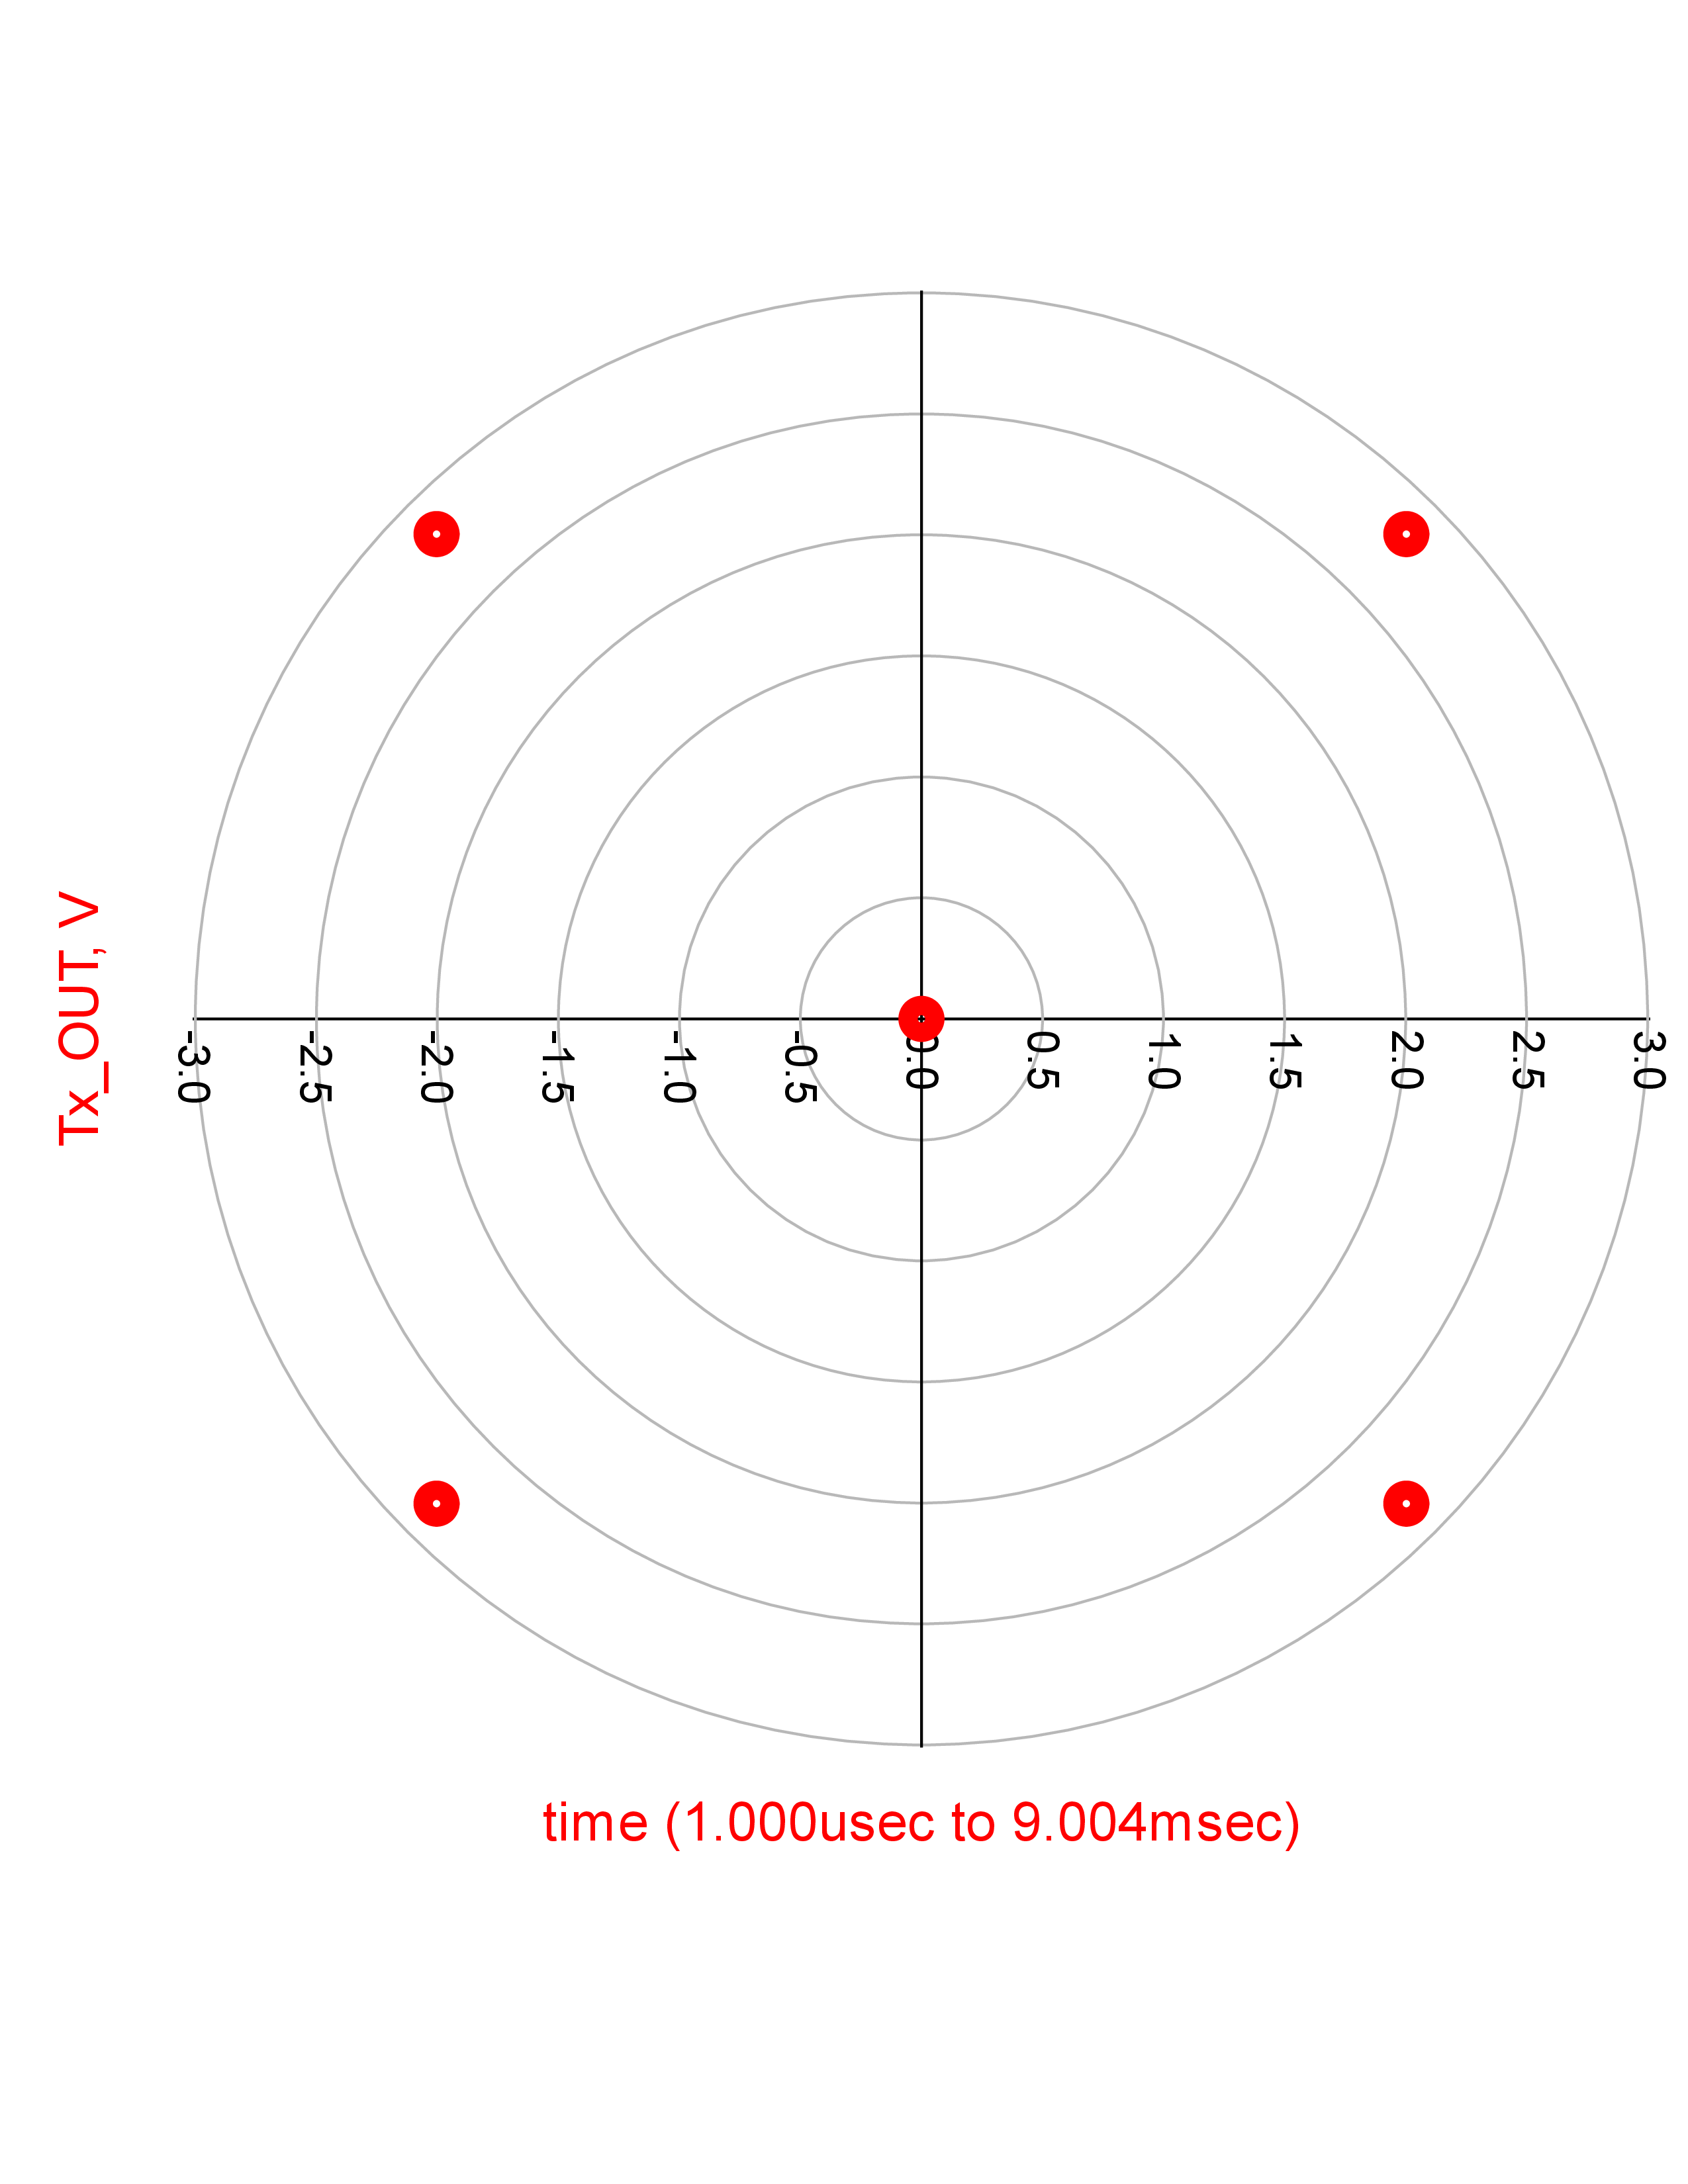
\includegraphics[width=.4\linewidth]{./primeiro_exp/img7.png}
\caption{Constelação QPSK, o ponto no centro da constelação aparece por problemas de casamento de impedância, os 4 pontos deslocados entre si de $90^o$ correspondem aos dados transmitidos, com os pontos no primeiro e terceiro quadrante correspondendo à uma via, e os pontos no segundo e quarto à outra}
\end{figure}


\chapter{Cálculo da BER - Experimento 2}
\section{Diagrama}
Neste segundo experimento, introduzimos ruído branco gaussiano dentro do canal e modelamos a atenuação sofrida pelo sinal durante o percurso, de forma que possamos observar a deterioração da Taxa de Erro de Bit e o espalhamento dos pontos da constelação QPSK. O esquema de modulação continua exatamente o mesmo.  

\begin{figure}
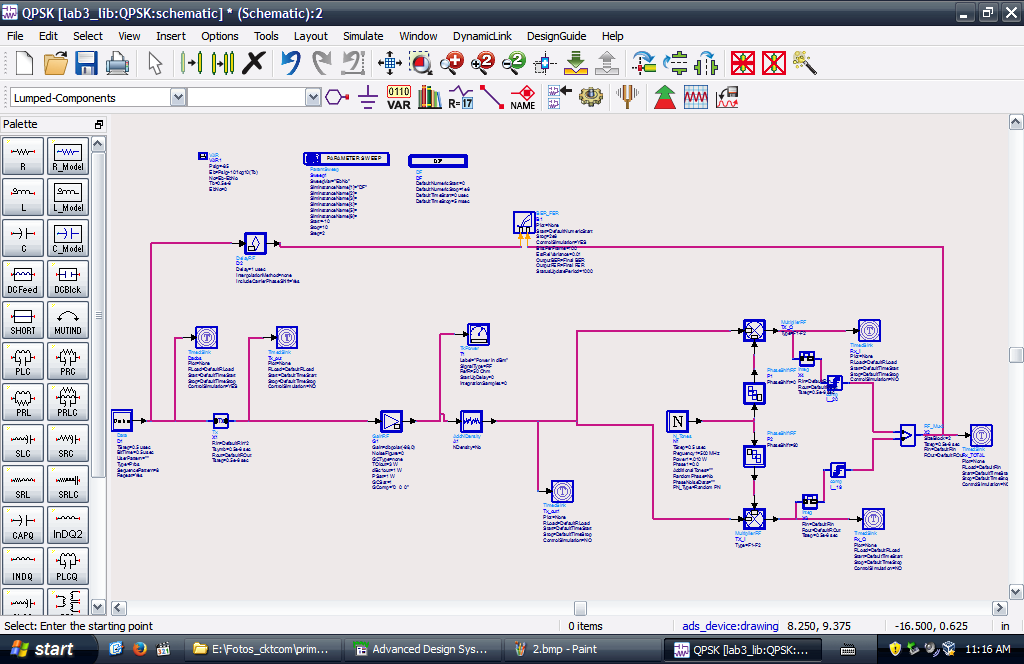
\includegraphics[width=.7\linewidth]{./segundo_exp/1.png}
\caption{Diagrama de Blocos Referente ao Segundo Experimento}
\end{figure}


\section{Resultados}
Como esperado, a medida que a relação $E_b/N_o$ que é análoga a SNR se deteriora, a Taxa de Erro de bit aumenta até se aproximar do seu valor limite de 0,5. A nuvem de pontos da constelação QPSK também fica cada vez mais espalhada na medida em que a relação se deteriora.


\begin{figure}
\centering
\begin{minipage}{.48\textwidth}
  \centering
  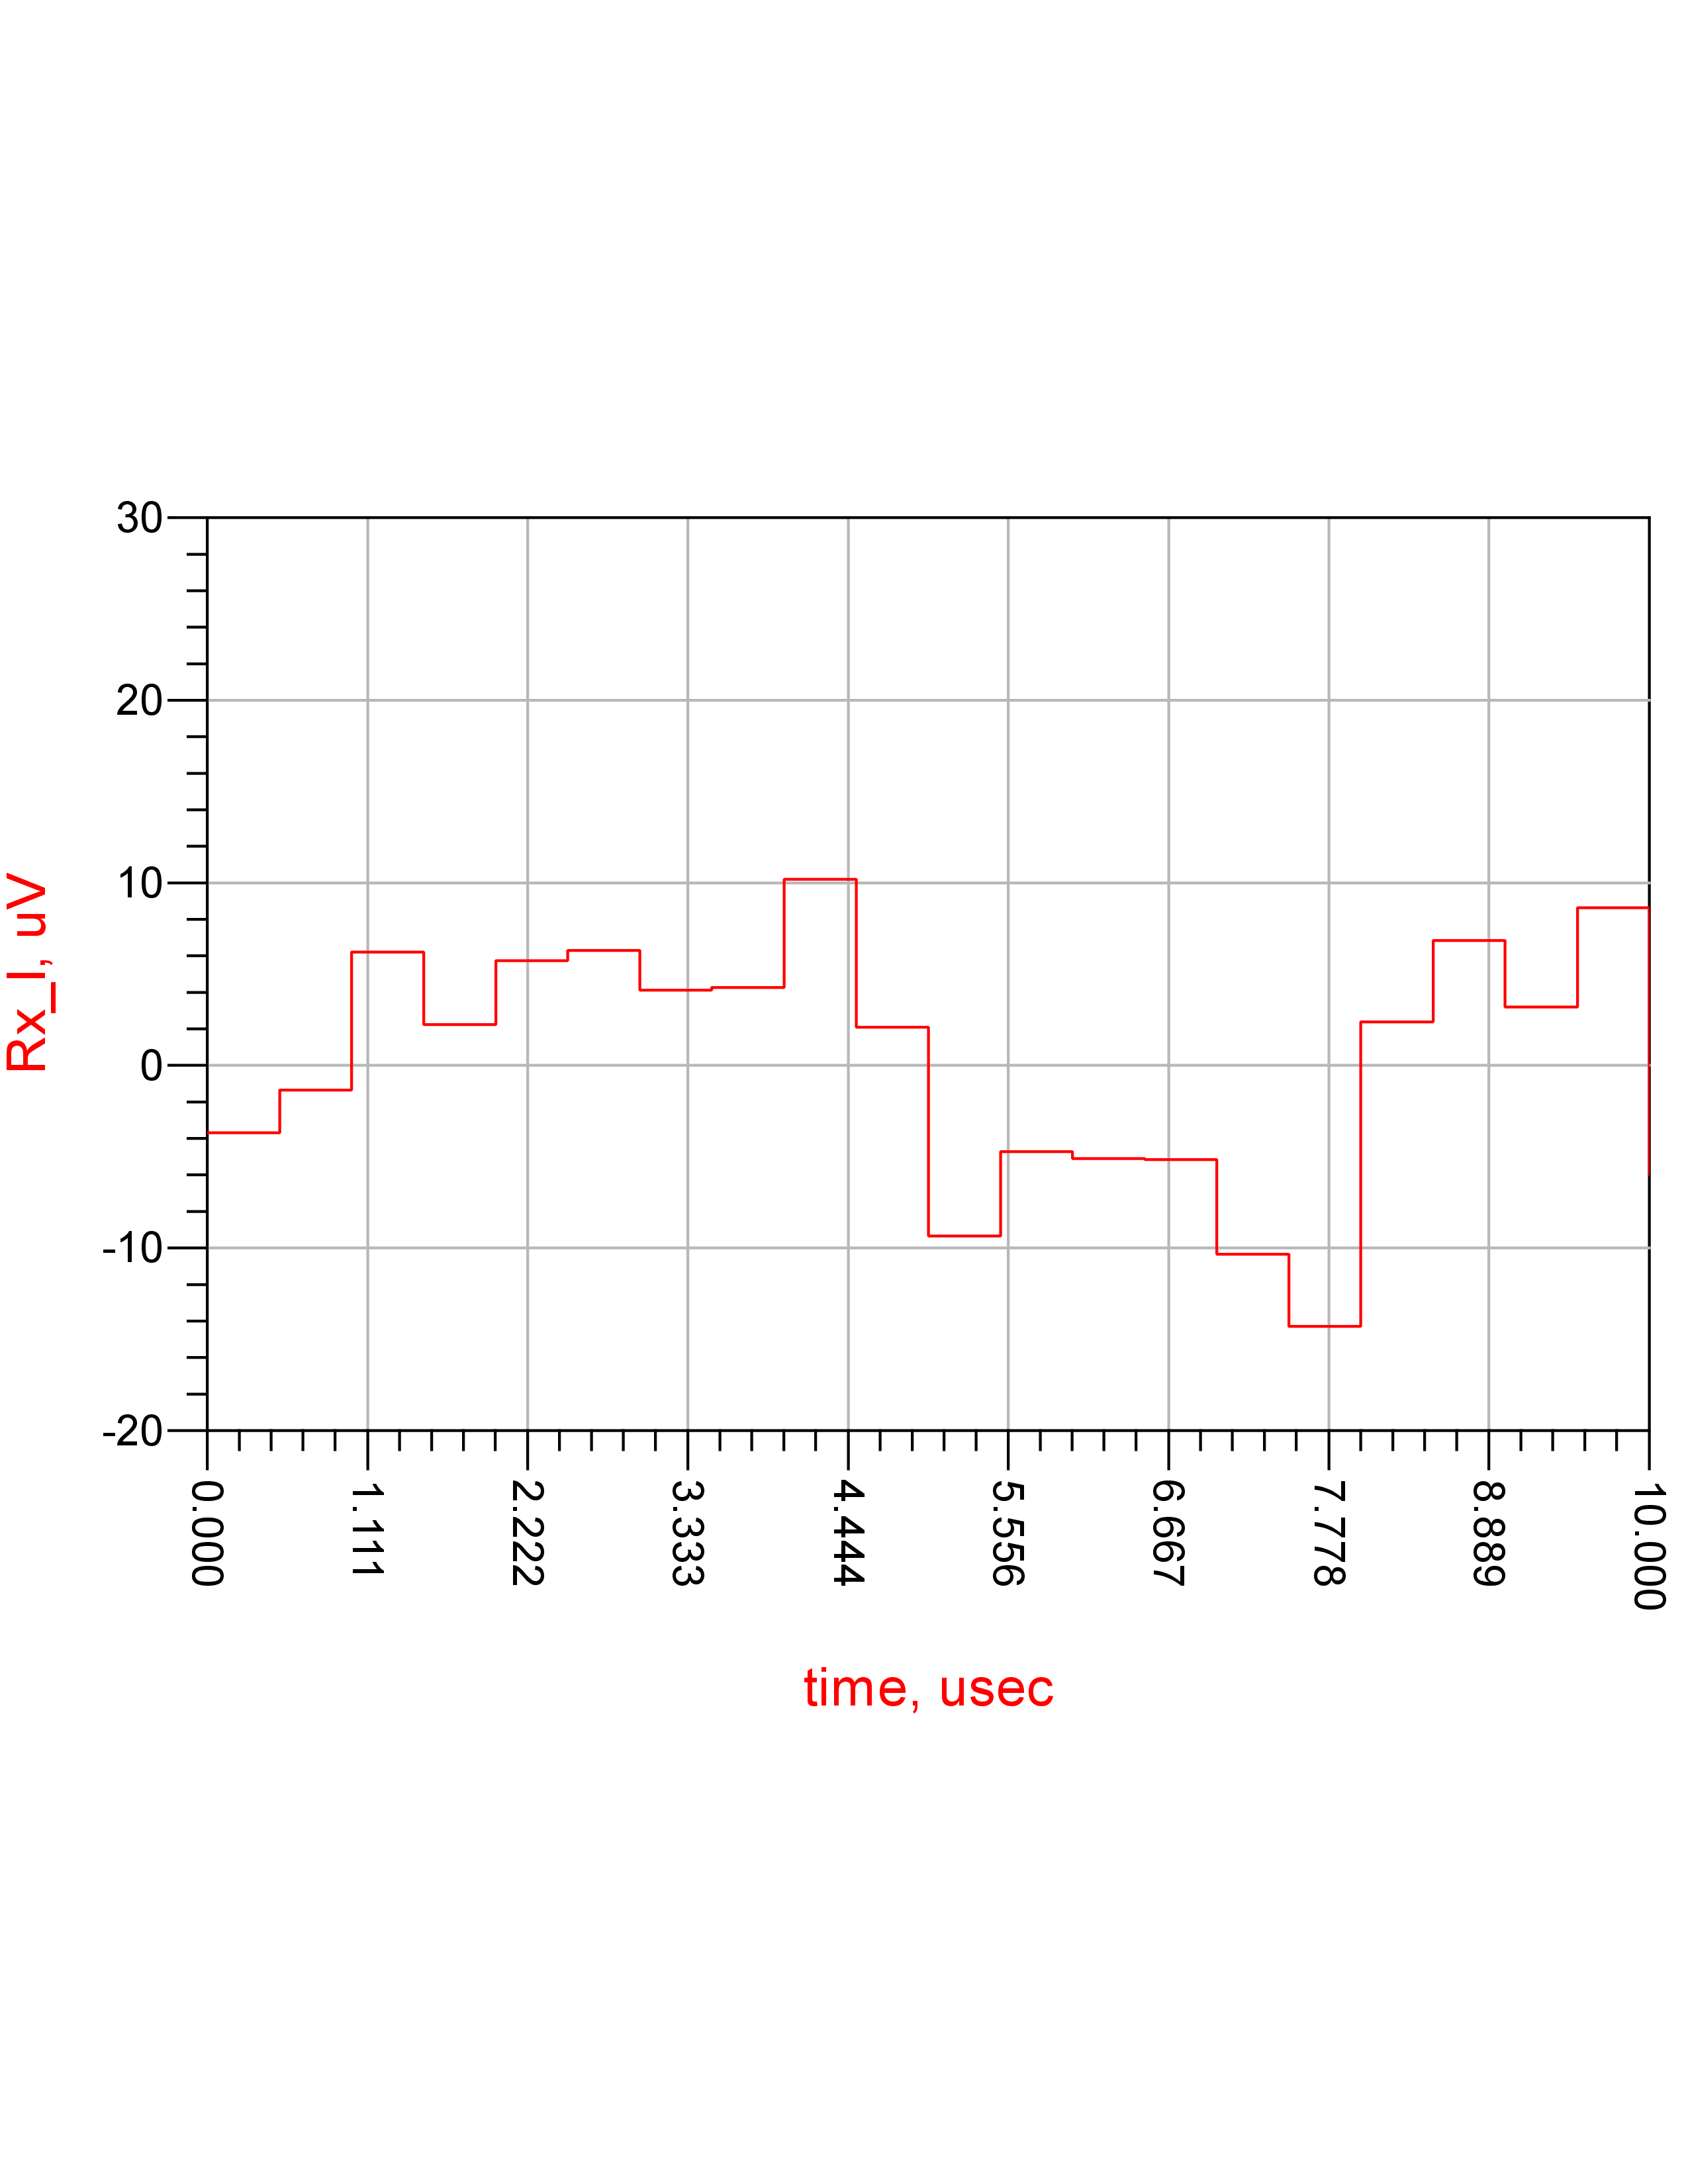
\includegraphics[width=\linewidth]{./segundo_exp/img4.png}
  \captionof{figure}{Via I, vemos os dados fortemente afetados pelo ruído e atenuação impostas}
  \label{fig:test38}
\end{minipage}%
  \hfill
\begin{minipage}{.48\textwidth}
  \centering
  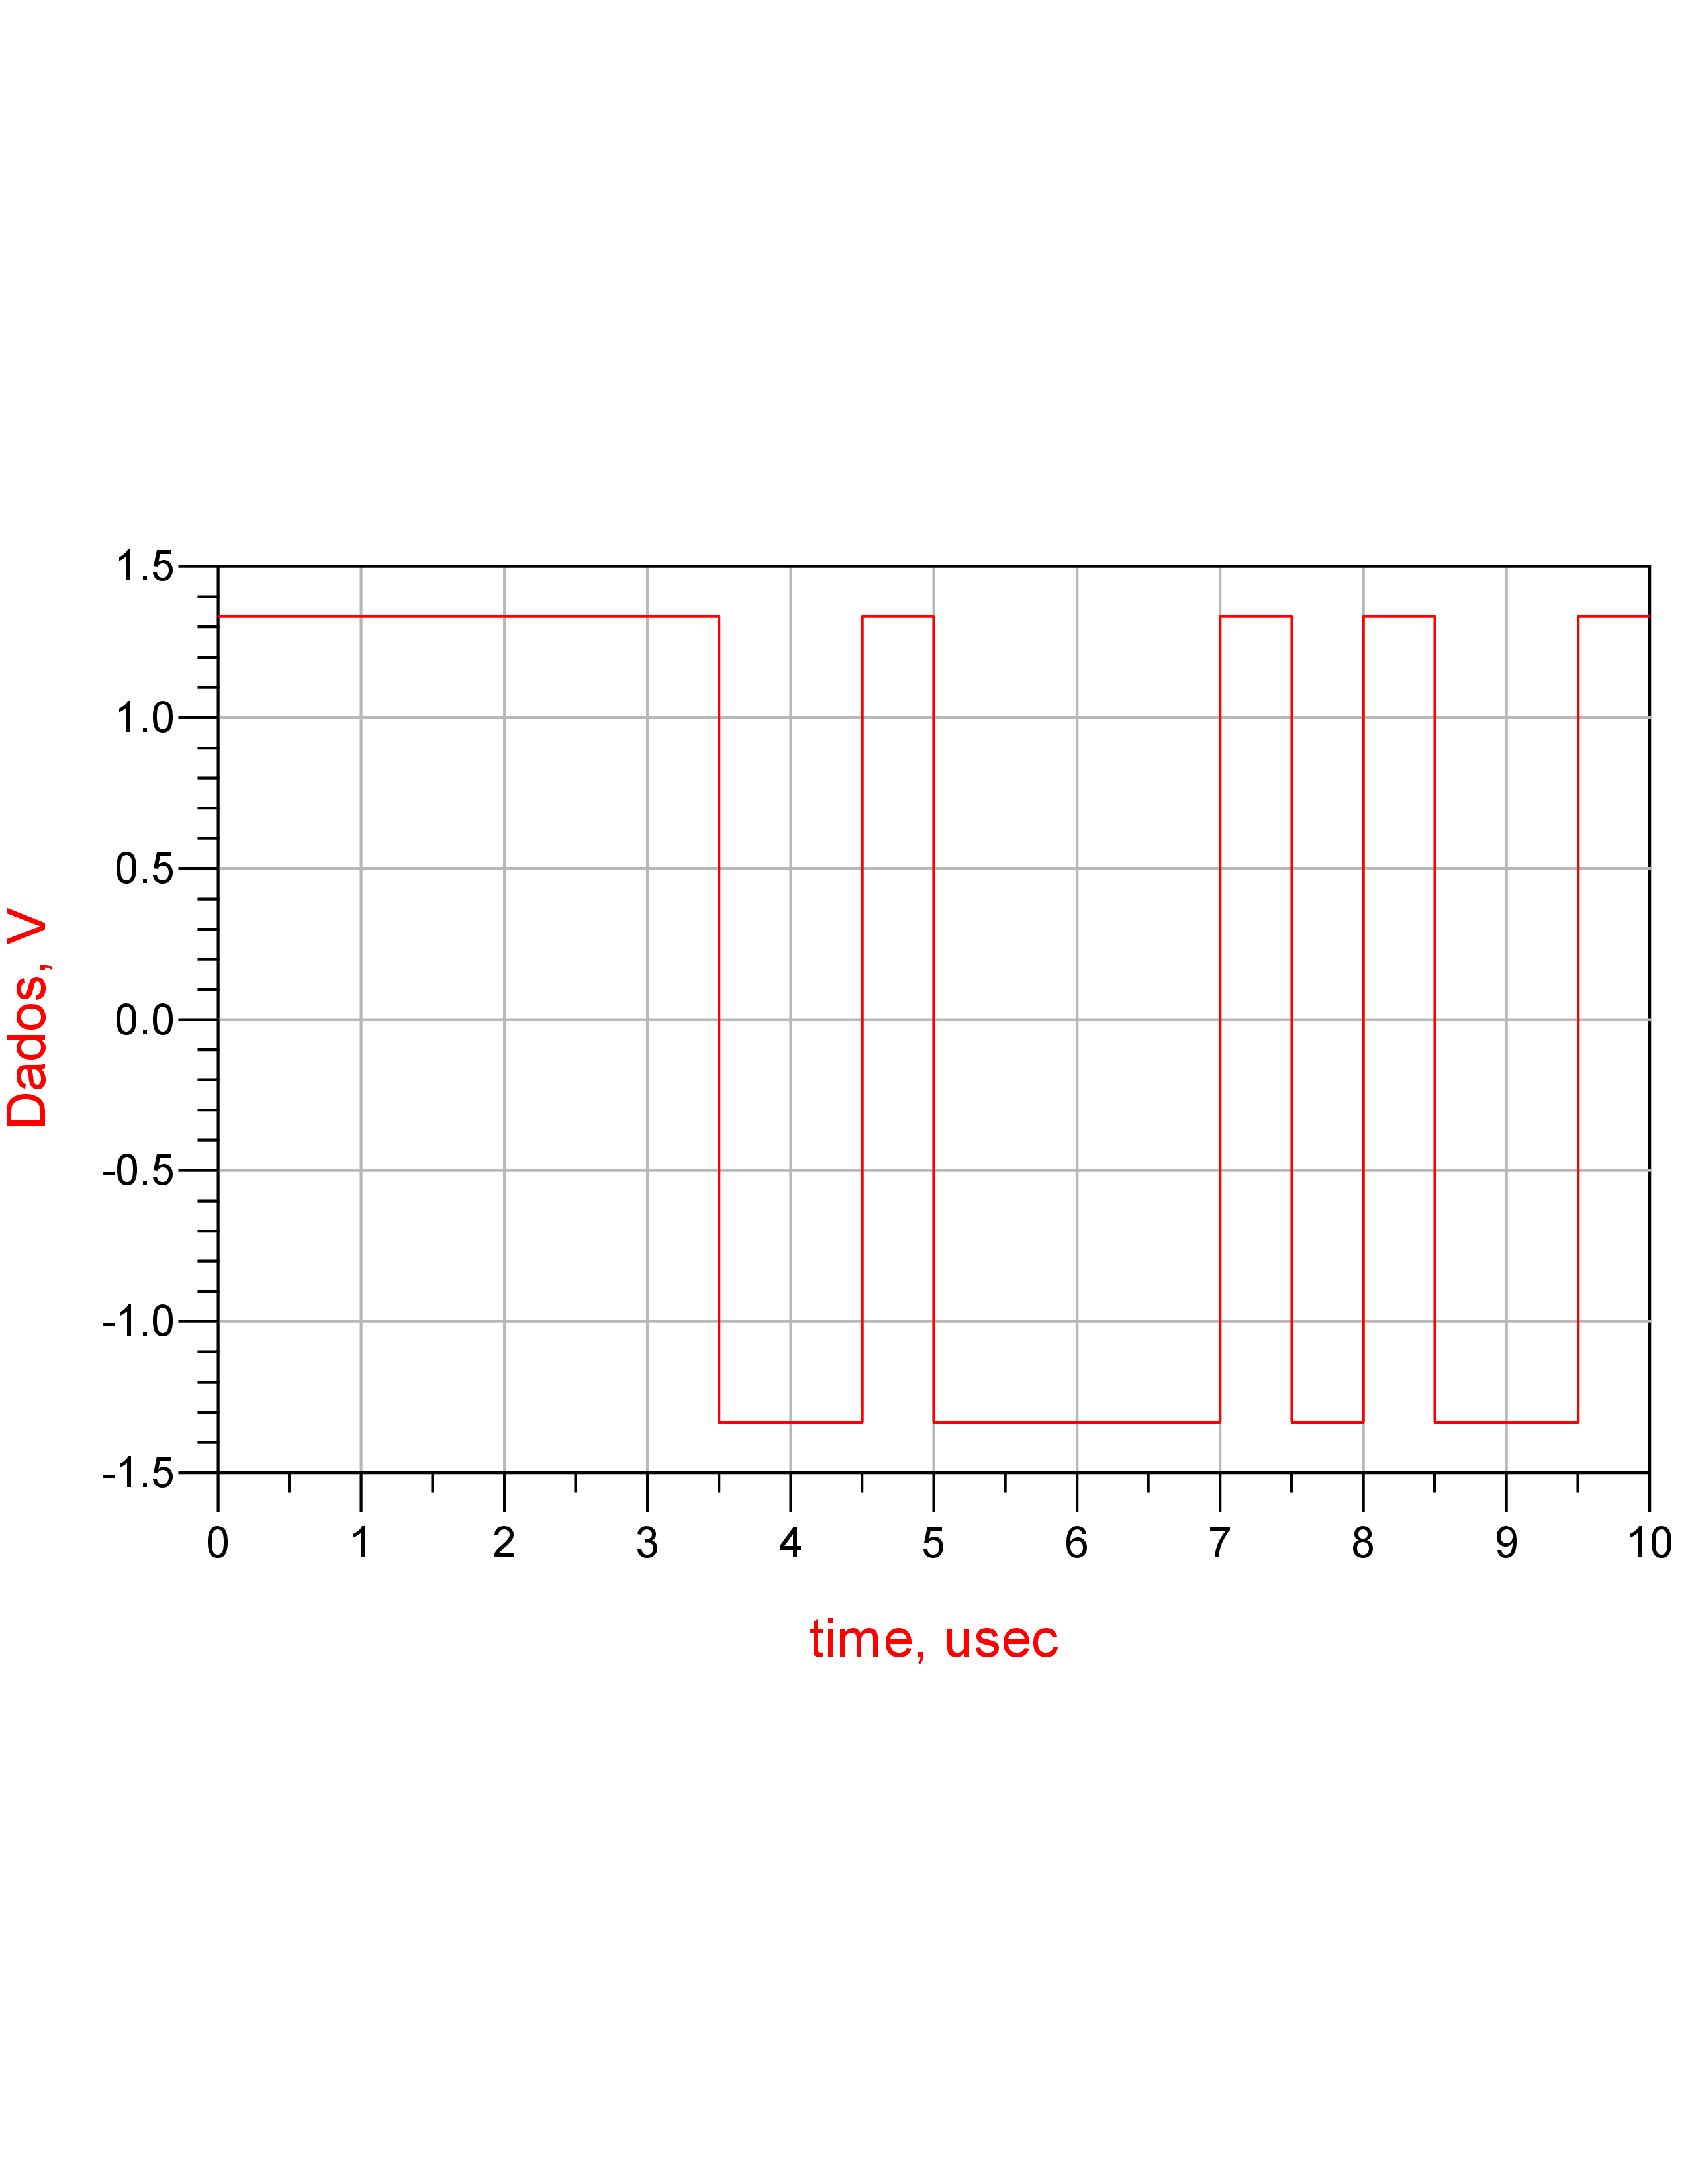
\includegraphics[width=\linewidth]{./segundo_exp/img1.png}
  \captionof{figure}{Dados gerados}
  \label{fig:test48}
\end{minipage}
\end{figure}
\begin{figure}
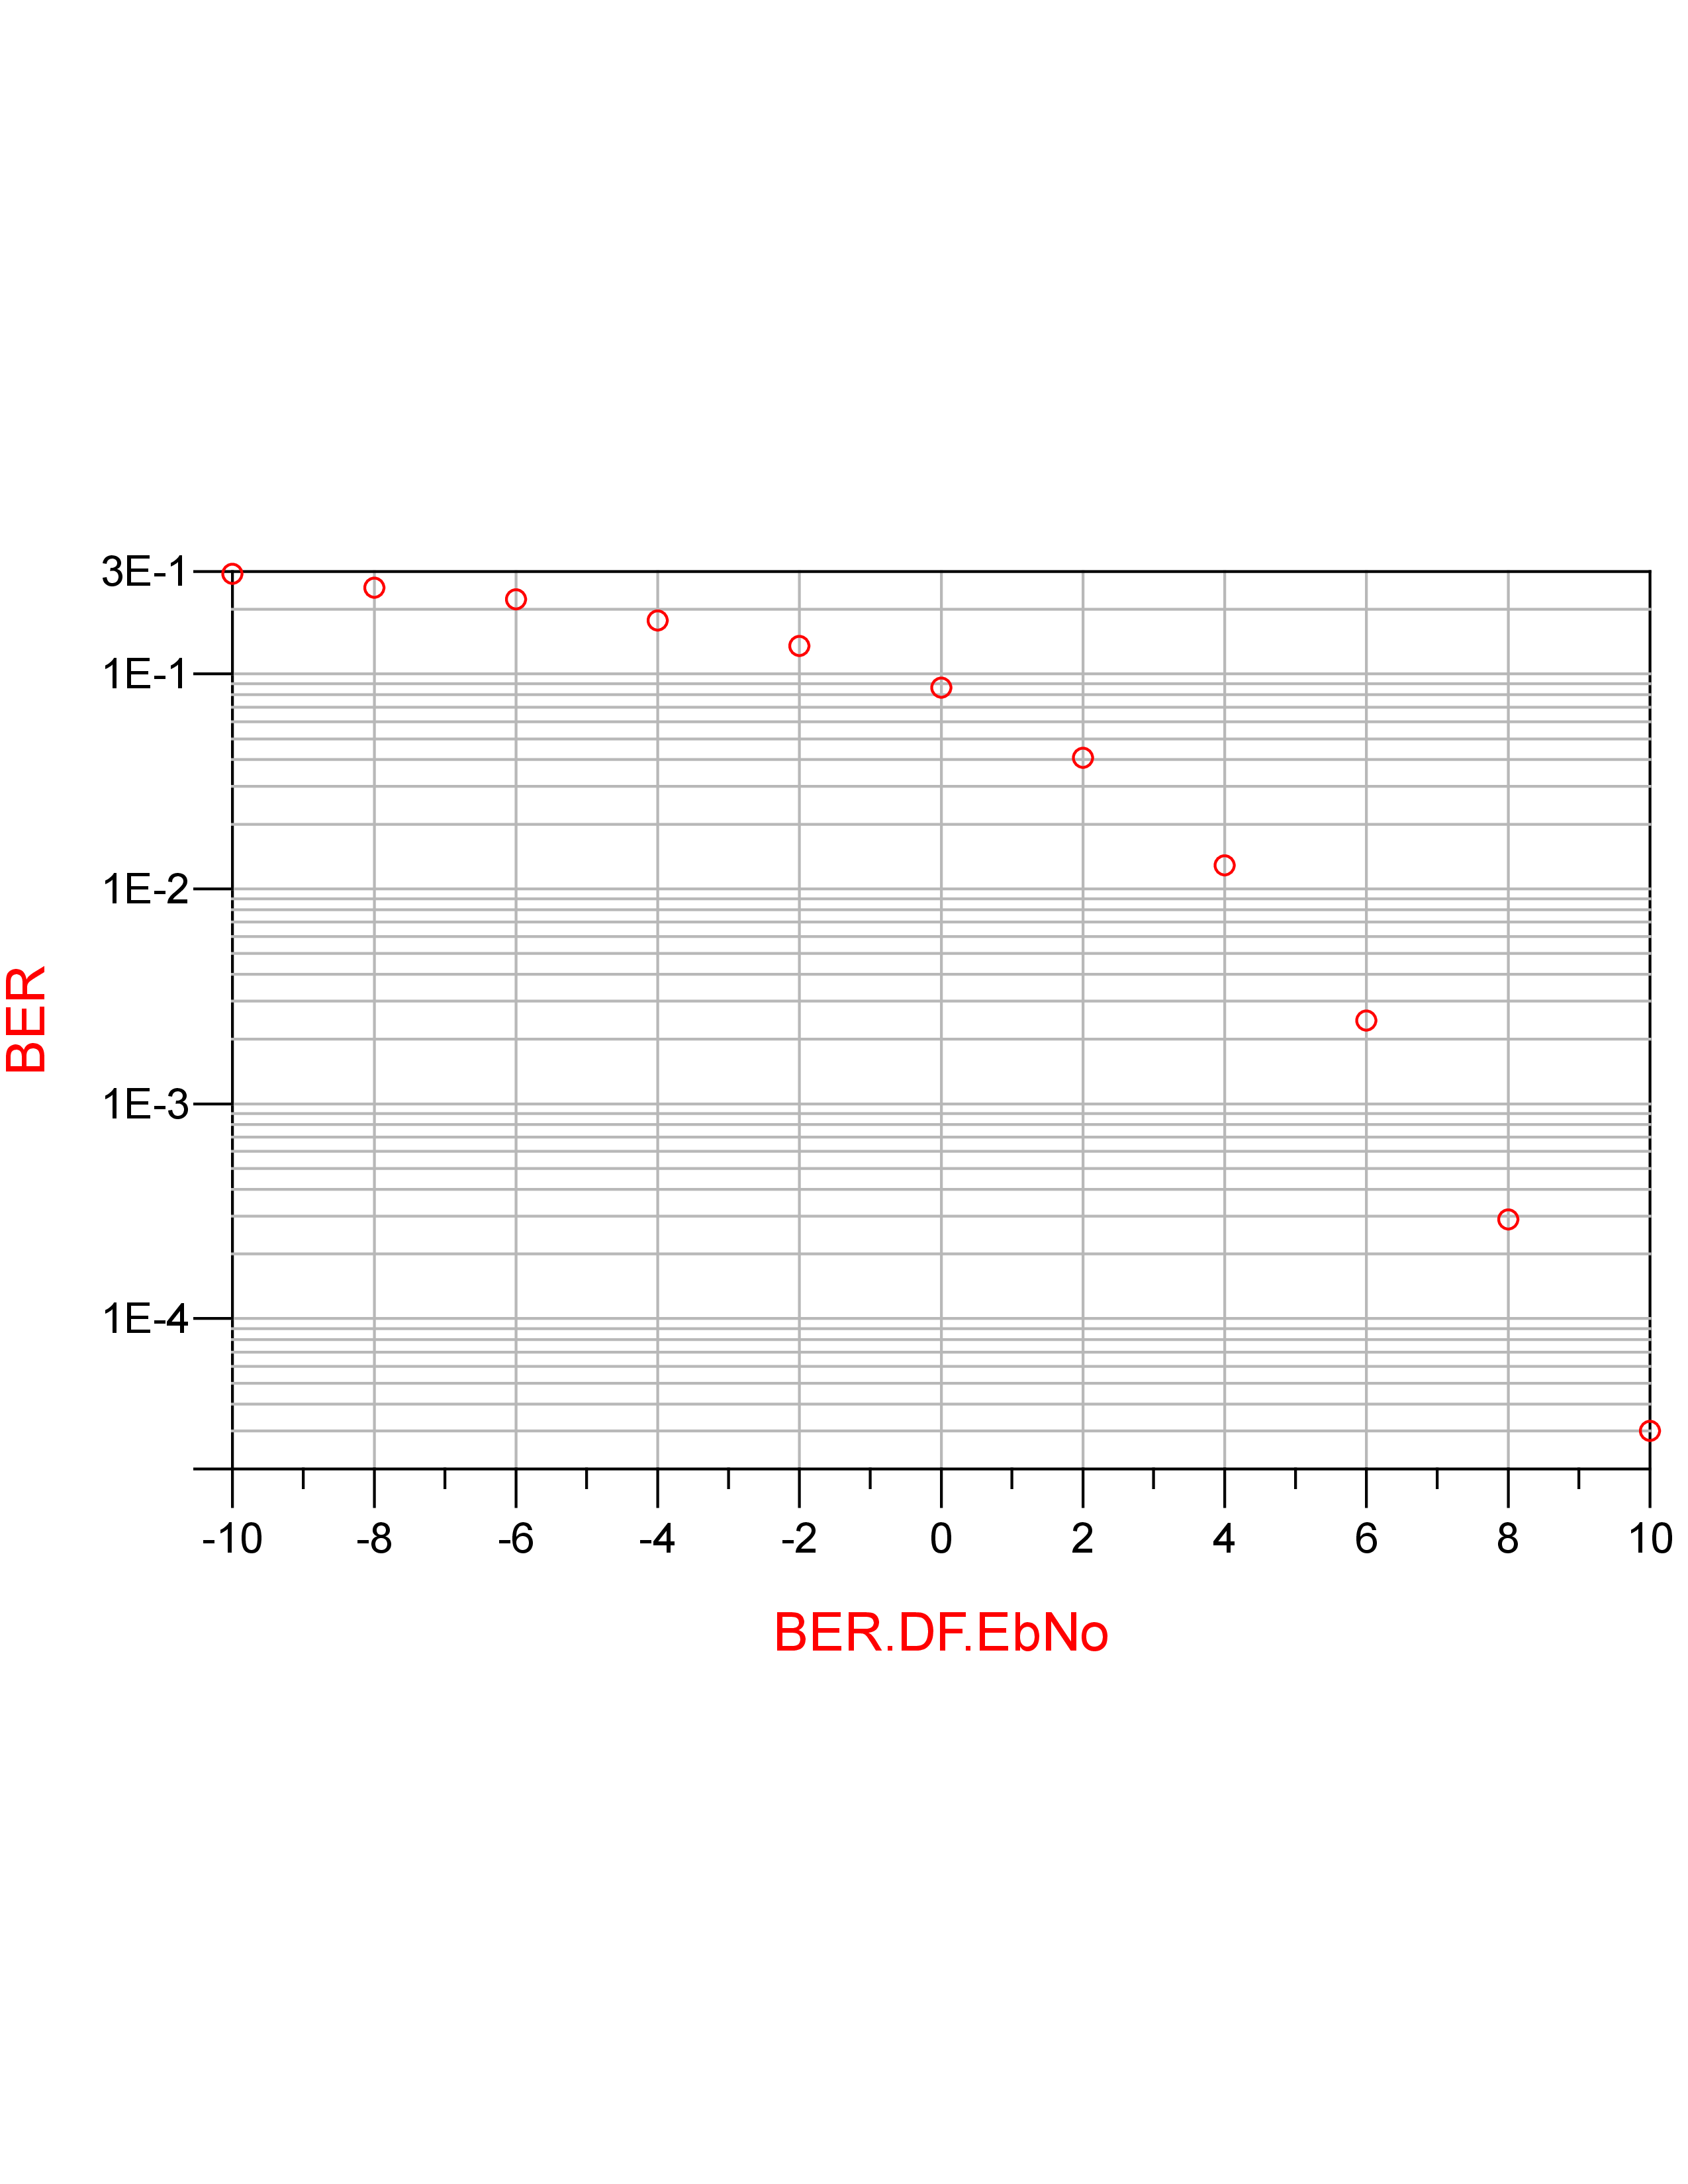
\includegraphics[width=.8\linewidth]{./segundo_exp/img7.png}
\caption{BER obtida com 1000000 pontos de simulação para vários valores de $E_b/N_o$. O valor obtido deve diferir levemente da curva teórica pois existe uma certa variância no número de bits que serão detectados de forma errada e esta variância deve pesar no cálculo da BER. A medida que o número de bits transmitidos aumenta, mais a curva obtida se aproxima da curva teórica}
\end{figure}
\begin{figure}
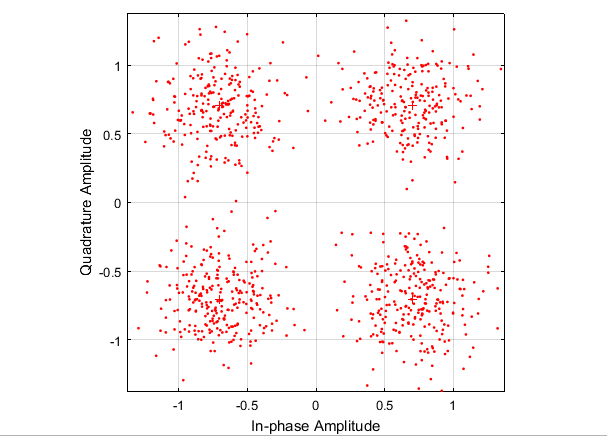
\includegraphics[width=.8\linewidth]{./segundo_exp/img8.png}
\caption{Espalhamento dos pontos da Constelação QPSK em forma de nuvem devido ao ruído AWGN. A figura utilizada foi gerada no MATLAB e é meramente ilustrativa pois nos esquecemos de retirar a figura correspondente ao ADS. Usamos 1000 pontos com uma SNR de 9dB de forma a ilustrar o conceito do surgimento de uma nuvem em torno dos pontos de referência da constelação.}
\end{figure}

\chapter{Conclusão}
Observamos a validade dos conceitos estudados em sala referentes à modulação QPSK, assim como a utilidade de ferramentas de design em alto nível tais como o ADS para sedimentar os conceitos e teoria referentes ao entendimento de sistemas de radiofrequência. 


\end{document}         